% siminos/CLE/CLE.tex
% $Author$ $Date$

                            \newif\ifdraft \newif\ifpaper
 \drafttrue\paperfalse       % draft version, commented
%  \draftfalse\papertrue     % final version, no comments
%%%%%%%%%%%%%%%%%%%%%%%%%%%%%%%%%%%%%%%%%%%%%%%%%%%%%%%%

% Predrag reorganized siminos/CLE/          2009-10-09
% Vaggelis created siminos/CLE/CLE.tex      2009-09-21
% Vaggelis created siminos/CLE              2009-02-05

%\documentclass[final,number]{elsarticle}
\documentclass[preprint,number,sort&compress]{elsarticle}

\usepackage{amsmath,amsfonts,amssymb,amsbsy,amscd}
\usepackage{ifthen}
\usepackage{graphicx}
\usepackage[dvips]{color}
\usepackage[dvips,colorlinks]{hyperref}
\input ../inputs/def        % TEMPORARY
\input inputs/defsCLE.tex   % eventualy merge used commanDs into inputs/defsCLE.tex

% Use the next command to get Bibliography header appear. The problem is a conflict
% between elsarticle and amsref over \bibsection command.
\newcommand\bibsection{%
  \section*{\bibname\markright{\MakeUppercase{\bibname}}}}

\begin{document}
\journal{Physica D}
\begin{frontmatter}

			\title{
Continuous symmetry reduction and return maps for higher-dimensional flows
			}
% Continuous symmetry reduction and return maps for high dimensional flows
% Continuous symmetry reduced return maps for high dimensional flows
% Returm maps of high dimensional flows with continuous symmetry:
%                                           I. Symmetry reduction
% Towards continuous symmetry reduction in high dimensional flows
\author{Evangelos Siminos}
\ead{siminos@gatech.edu}
\author{Predrag Cvitanovi\'c}
\address{Center for Nonlinear Science,
School of Physics, Georgia Institute of Technology,
Atlanta, GA 30332-0430}
%\homepage[]{Your web page}
%\thanks{}
%\altaffiliation{}


\date{\today}

        \begin{abstract}
\input abstract
        \end{abstract}

\begin{keyword}
continuous symmetry reduction,
relative equilibria,
relative periodic orbits,
return maps,
slices,
moving frames,
Hilbert polynomial bases
\PACS 05.45.-a \sep 47.27.ed \sep 42.65.Sf
% 05.45.-a 	Nonlinear dynamics and chaos
% 05.45.Jn 	High-dimensional chaos
% 47.10.Fg 	Dynamical systems methods (in Fluid Mechanics)
% 47.27.ed 	Dynamical systems approaches (turbulent flows)
% 47.52.+j 	Chaos in fluid dynamics
% 42.65.Sf 	Dynamics of nonlinear optical systems; optical instabilities,
% 		optical chaos and complexity, and optical spatio-temporal dynamics
\end{keyword}
\end{frontmatter}

\section{\label{s:intro} Introduction}
    \PC{please keep improving abstract, intro and conclusions at each proofreading.
    \\
    remove PC\{\} and PCedit\{\} after you have accepted/edited them}
    \input intro

% \section{\label{s:symDyn} Symmetries of dynamical systems}
    \input symDyn

% \subsection{\label{s:introCLE} An example: \CLe}
    % siminos/CLE/introCLE.tex
% $Author$ $Date$

% introducing CLe
% from siminos/thesis/lasersSym.tex

\CLe\ (henceforth CLE) were introduced by Gibbon and McGuinness\rf{GibMcCLE82} as a low-dimensional model
of baroclinic instability in the atmosphere.
As the name suggests they turned out to be a complex generalization
of Lorenz equations\rf{lorenz}:
\beq
\index{Complex Lorenz equations}
\begin{split}
 \dot{x} &=-\sigma x+ \sigma y \cont
 \dot{y} &=(\rLor-z)x-a y \cont
 \dot{z} &= \frac{1}{2}\left(x y^*+x^*y\right)-b z\,,
 \label{eq:CLe}
\end{split}
\eeq
where $x,y$ are complex variables, $z$ is real, while the
parameters $\sigma,\,b$ are real and $\rLor=\RerCLor+i
\ImrCLor$, $a=1-i e$ are complex.

It can easily be checked that \cLe\ are 
equivariant under the one parameter rotation
group $\Un{1}\cong\SOn{2}$ acting by
\beq\label{eq:SO2cle}
	(x,\,y,\,z)\mapsto (e^{i\theta}x,\,e^{i\theta}y,\,z)\,,\ \theta\in[0,2\pi]\,,
\eeq

Ning and Haken\rf{NingHakenCLE90} have shown
that equations isomorphic to \cLe\ also appear as a
truncation of Maxwell-Bloch equations describing a single
mode, detuned, ring laser.
%with $x,y$ and $z$
%proportional to electric field, polarization and population inversion, respectively.
They set $e+\ImrCLor=0$ so that a detuned
\eqv\ exists.
    \ES{This assumption is questionable unless it
is forced by the physics of the problem, which I cannot
follow very well. It leads to non-generic bifurcation
behavior, while one would like a model of a physical system
to be robust under perturbations (of the model). Furthermore,
the fact that the Hopf cycle in the general case is an
$\SOn{2}$-orbit has gone unnoticed. The \reqv\ can be
interpreted as an \eqv\ in a rotating frame and the measured
electric field of the laser would be the same in both cases.
    }
In contrast Bakasov and Abraham\rf{BakasovAbraham93} only require
that a \emph{relative equilibrium}, see \refsect{s:symDyn}, exists
and show that one can use
\CLe\ with $\ImrCLor=0$ and $e \neq 0$ to describe detuned lasers.
Here we follow the choice of Bakasov and Abraham, since as shown by Krupa\rf{Krupa90} 
it corresponds to the generic bifurcation senario in a system with the symmetry
of CLE. Moreover, in all numerical examples
that follow, the parameters will be set to the Lorenz values
$\RerCLor=28,\, b=8/3,\, \sigma=10$, with the ``detuning'' $e=1/10$ unless explicitly
stated otherwise. Note that $e$, although related to detuning in Maxwell-Bloch equations
is not directly proportional to it\rf{BakasovAbraham93}.

\PublicPrivate{}{
 \refFig{fig:CLE} illustrates the need
 to project dynamics on \reducedsp: Dynamics is organized by
 the interplay of the stable and unstable manifolds of \eqv\
 \EQV{0} and \reqv\ \REQV{}{1} but the dynamics along the
 direction of rotation blur the picture and the notion of
 recurrence becomes relative. We will present various
 approaches to orbit space reduction in the following.
% sections.
    }

    \ES{move to elsewhere: ``
The lowest level of organization of the
familiar (real) Lorenz system that does not posses a
continuous symmetry can be
understood\rf{DasBuch,SiminosThesis} in terms of the unstable
manifolds of the equilibrium at the origin and the two
(discrete-symmetry-related) equilibria $\EQV{1,2}$. In the
case of {\cLe}  the origin \EQV{0} is an \eqv\ of
\refeq{eq:CLe} for any value of the parameters. As shown in
\refref{FowlerCLE82} it is stable for $0<\RerCLor<\rho_{1c}$
and unstable for $\rho_{1c}<\RerCLor$, where
\beq
	\rho_{1c} = 1 + \frac{(e+\ImrCLor)(e-\sigma \ImrCLor)}{(\sigma+1)^2}\,.
\eeq
At bifurcation a pair of eigenvalues crosses the imaginary axis with imaginary part:
\beq
	\omega_c = \frac{\sigma (e + \ImrCLor)}{\sigma+1}\,.
	\label{eq:omegaCLE}
\eeq
and a \emph{relative equilibrium} \REQV{}{1}, an equilibrium
in a frame rotating with constant angular velocity is born.
Alternatively we might say that a relative equilibrium is a
periodic orbit that is invariant (as a set) under the action
of $\LGelement{l_p}\in\Group$ for any $l_p$.
    \ES{this implies constant angular velocity by
    equivariance.}
    \ES{Does not fit here, but keep: For $e+\ImrCLor=0$ the
    relative equilibrium degenerates to an \SOn{2}-orbit of
    \eqva\rf{FowlerCLE82}, since $\omega_c =0$.}
As we will see in \refsect{s:StabReq}, \REQV{}{1} of {\cLe}
for the parameter set we study here is unstable with one
complex expanding eigenvalue. Yet, being a periodic orbit,
its unstable manifold is three-dimensional, with one
eigendirection corresponding to the direction of $\vf$ which
also coincides with the direction of rotations of the system.
In \reffig{fig:CLE} we plot one trajectory on the unstable
manifold of \REQV{}{1}. While it spirals away from
$\REQV{}{1}$ it also ``drifts'' along the direction of
rotations of the system. This drifting motion obscures
understanding of the stretching mechanism along the expanding
eigendirection and subsequently the folding of the unstable
manifold back to itself.
    ''} %end \ES{move to elsewhere: ``
%
%%%%%%%%%%%%%%%%%%%%%%%%%%%%%%%%%%%%%%%%%%%%%%%%%%%%%%%%%%%%
\begin{figure}[ht]
\begin{center}
  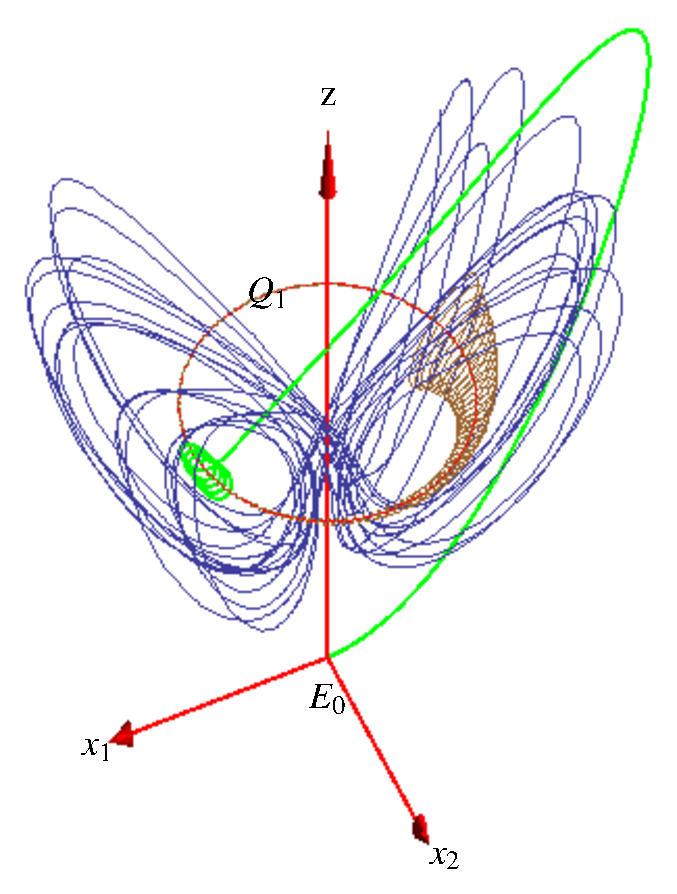
\includegraphics[height=0.25\textheight]{../figs/CLE}
\end{center}
\caption[Complex Lorenz flow phase space]
{ \Statesp\ portrait of \cLe\ dynamics for $e=1/10,\,
\ImrCLor=0$. Plotted are \reqv\ \REQV{}{1} (red), its unstable
manifold (brown), \eqv\ \EQV{0}, a representative of its
unstable manifold (green), 3 repetitions of \rpo\
``01''(magenta) and a generic orbit (blue).}
\label{fig:CLE}
\end{figure}
%%%%%%%%%%%%%%%%%%%%%%%%%%%%%%%%%%%%%%%%%%%%%%%%%%%%%%%%%%%%
%


\ES{move elsewere: The next (or a complimentary) level of organization of (real)
{\Le} attractor is provided by the dense set of \po s
embedded in it\rf{DV03,DasBuch}. In {\cLe} a secondary
bifurcation from \REQV{}{1} is expected, according to Krupa's
theorem\rf{Krupa90}, to result in \emph{relative periodic
orbits} that satisfy
\beq
	\LGelement{l_p}x(t+T_p)=x(t)\,,
\eeq
{\ie} they ``return'' after a time period $T_p$ to a point
that maps to the initial one under a group transformation
$\LGelement{l_p}$ with group parameter period $l_p$. A {\rpo}
of {\cLe} is shown in \reffig{fig:CLE} as its iterations fill
a torus. Therefore we see that in systems with continuous
symmetry we have to account for tori instead of {\po s} as
the organizational blocks of the attractor.
}



\subsection{\CLe\ \reqva}

To find the location of the \reqv\ it is convenient to work
on polar coordinates defined by $x=r_1 e^{i \phi_1},\,y=r_2
e^{i \phi_2}$. Equations \refeq{eq:CLe} take the form
    %PC: Rebecca and I rederived these: they check.
\beq
\begin{split}
	\dot{r}_1 &=-\sigma (r_1 - r_2\cos\phi) \cont
	\dot{r}_2 &=-r_2 + r_1(\RerCLor -z)(\cos\phi-\ImrCLor\sin\phi) \cont
	\dot{z} &=  -b z+r_1 r_2\cos\phi \cont	
	\dot{\phi} &=-e-\frac{\sigma r_2 \sin\phi}{r_1}-\frac{r_1(\RerCLor-z) (\ImrCLor\cos\phi+\sin\phi) }{r_2}\,,
	\label{eq:CLePolar}
\end{split}
\eeq
where $\phi=\phi_1-\phi_2$ and the evolution equations for
$\phi_1,\phi_2$ are given by
\beq
\begin{split}
	\dot{\phi}_1 &=-\frac{\sigma r_2 \sin\phi}{r_1}\cont
	\dot{\phi_2} &= e +\frac{r_1\left( (\RerCLor -z)\sin\phi+\ImrCLor\cos\phi\right)}{r_2}\,.
	\label{eq:CLeAngl}
\end{split}
\eeq

For simplicity we now turn to the ``laser case''
$e\neq0,\;\ImrCLor=0$; in the numerical examples we set the
detuning to $e=1/10$.

The condition for a \reqv~ is that all time derivatives in
\refeq{eq:CLePolar} vanish from which we get
% Explicit form here, simplified in terms of z component below
% \beq
% \begin{split}
% 	z &= -\frac{e^2}{(\sigma +1)^2}+\RerCLor -1\cont
% 	r_2 &= \frac{\sqrt{-b \left(e^2+(\sigma +1)^2\right)\left(e^2-(\RerCLor -1) (\sigma +1)^2\right)}}{(\sigma+1)^2}\cont
% 	r_1 &= \frac{\sqrt{-b \left(e^2-(\RerCLor -1) (\sigma +1)^2\right)}}{\sigma +1}\cont
% 	\Phi &= -\cos ^{-1}\left(\frac{\sigma +1}{\sqrt{e^2+(\sigma +1)^2}}\right)
% \end{split}
% \eeq
\beq
\begin{split}
	z^{(1)} &= \frac{-e^2+(\RerCLor -1)(\sigma +1)^2}{(\sigma +1)^2}\cont
	r_1^{(1)} &= \sqrt{b z^{(1)}}\cont
	r_2^{(1)} &= \sqrt{b \left(e^2+(\sigma +1)^2\right)z^{(1)}}\cont
	\phi^{(1)} &= -\cos ^{-1}\left(\frac{\sigma +1}{\sqrt{e^2+(\sigma +1)^2}}\right)
\end{split}
\eeq
Substituting in \refeq{eq:CLeAngl} we get $\dot{\phi}_1=\dot{\phi}_2=e \sigma/(1 + \sigma)\neq 0$ for $e\neq0$
and thus we have indeed a \reqv, not a group orbit of \eqva.

Calculation  in polar coordinates $r_1,r_2,\phi,z$ of stability eigenvalues for \REQV{}{1}
for the set of parameters we use here yields
\beq
	\eigRe[1]\pm i\eigIm[1]= 0.0938\pm 10.1945i,\,
    \eigExp[3]=-11.0009,\, \eigExp[4]= -13.8534\,.
	\label{eq:CLeREQBstab}
\eeq


% \section{\label{s:symSol} Solutions of systems with continuous symmetry}
   % siminos/CLE/symSol.tex
% $Author$ $Date$

\section{\label{s:symSol} Symmetries of solutions}

In order to explore the implications of equivariance for the
solutions of dynamical equations,  we start by examining the
way a compact Lie group acts on \statesp\ \pS. The
\emph{group orbit} or the \emph{$\Group$-orbit} of the point
$\ssp \in \pS$ is the set
\beq
    \pS_\ssp = \{\LieEl\,\ssp \mid \LieEl \in {\Group}\}
\ee{GroupOrb}
of all \statesp\ points into which $\ssp$ is mapped under the
action of $\Group$.
The \emph{symmetry} $\stab{\ssp}$ (\emph{isotropy} or
\emph{stabilizer} group) of a \statesp\ point $\ssp$ is the
largest subgroup of $\Group$
\beq
\stab{\ssp} =\{\LieEl \in \Group: \LieEl \ssp = \ssp \}
\ee{def:isotr}
that leaves $\ssp$ fixed.
The \emph{symmetry} $\stab{X}$ of a set $\pS_X \in \pS$ is
the largest subgroup  of $\Group$ that leaves $\pS_X$
invariant as a set:
\[
	\stab{X}= \{\LieEl: \LieEl \, \pS_X = \pS_X\}
\,.
\]
If $\stab{p}$ is a symmetry, intrinsic properties of a
solution $\pS_p$ (such as \eqv\ or a cycle stability
eigenvalues, period, Floquet multipliers) evaluated anywhere
along its $\stab{p}$-orbit are the same. A symmetry thus
reduces the number of inequivalent solutions. So we also need
to describe the symmetry of a \emph{solution}, as opposed to
\refeq{eq:equivFinite}, the symmetry of the \emph{system}.

The \emph{\fixedsp} $\Fix{\Subgroup}$ of a subgroup
$\Subgroup\subset\Group$ is the subspace of $\pS$ containing
all fixed points of $\Subgroup$:
\[
	\Fix{\Subgroup}=
      \{\ssp\in\pS,\,\LieEl\in\Subgroup \,|\,
        \LieEl \ssp = \ssp \}
\,.
\]
The physical importance of \fixedsp s lies in the fact that
they are invariant under $\Group$-equivariant
dynamics\rf{golubitsky2002sp},
\[
 f^\tau\left(\Fix{\Subgroup}\right)\subseteq \Fix{\Subgroup}
\]
and thus \emph{flow} invariant for all times $\tau$.
Therefore if $\ssp(\tau)$ is a solution of an equivariant ODE,
then its symmetry $\stab{\ssp(\tau)}=\stab{\ssp(0)}$ is
preserved for for all times.

%
%%%%%%%%%%%%%%%%%%%%%%%%%%%%%%%%%%%%%%%%%%%%%%%%%%%%%%%%%%%%%%%%
% hand-drawn in dasbuch/book/FigSrc/xfig/rpo.fig
\begin{figure}[ht]
 (\textit{a})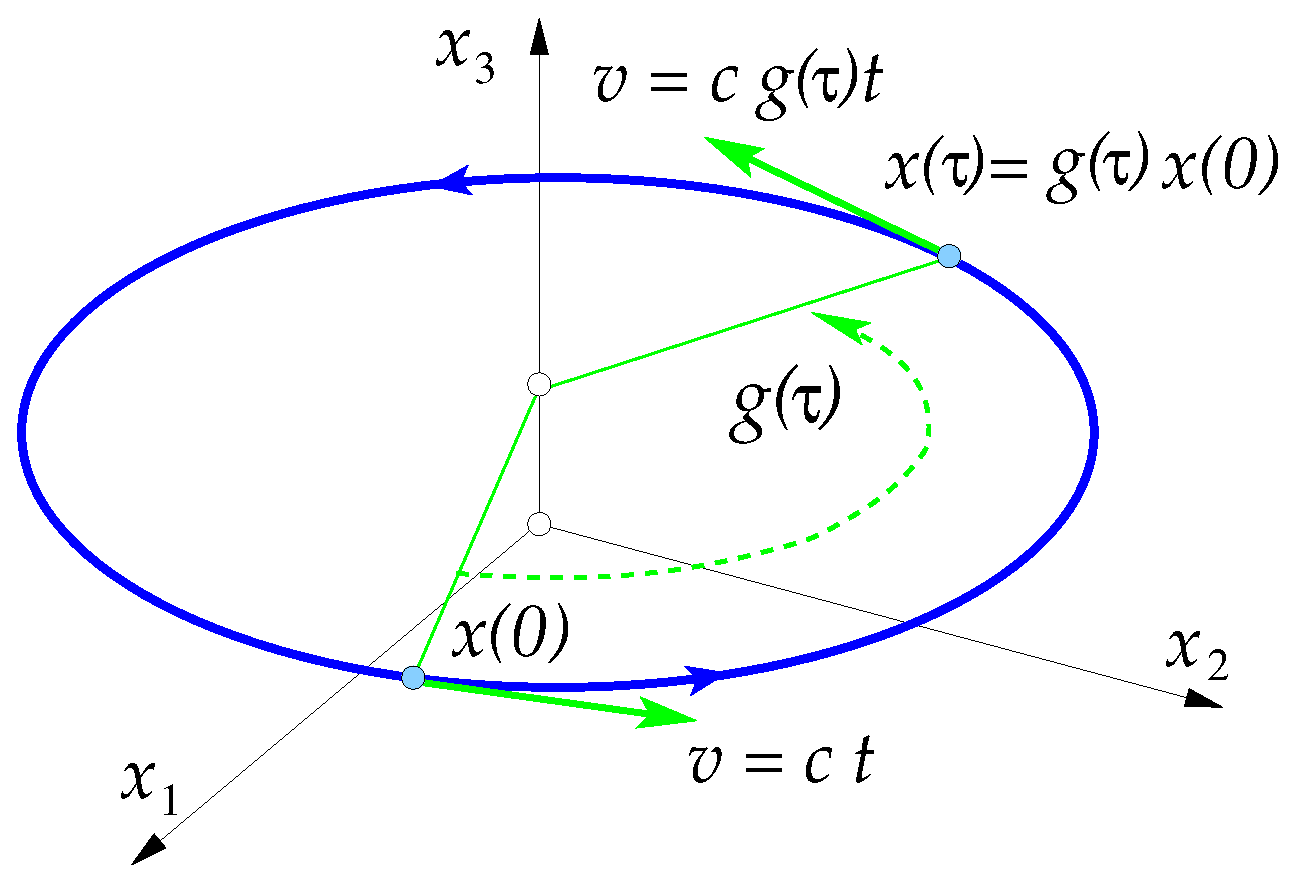
\includegraphics[width=0.40\textwidth]{../Fig/reqv.eps}
~(\textit{b})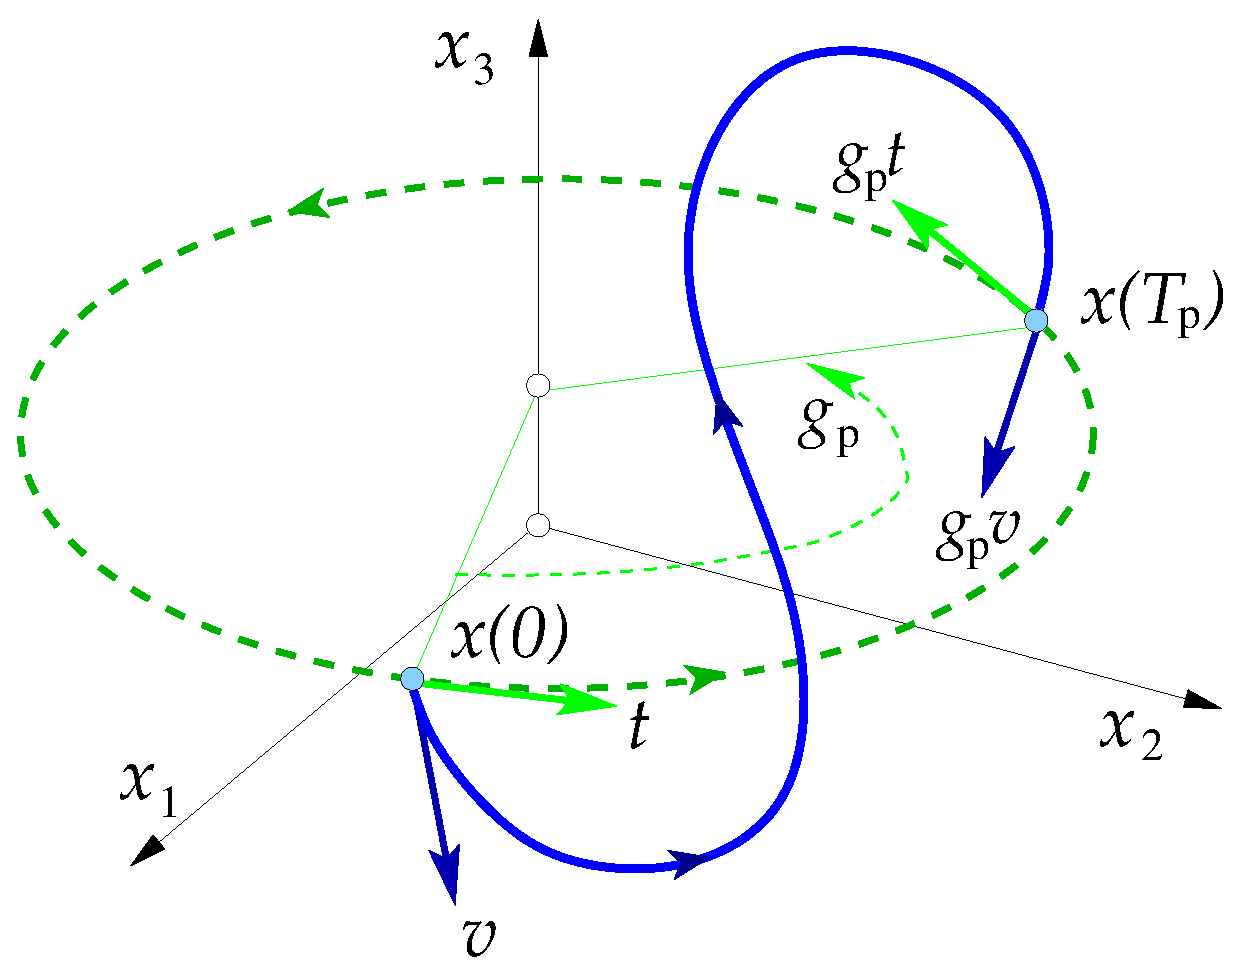
\includegraphics[width=0.40\textwidth]{../Fig/rpo.eps}
\caption{
(a) A {\em \reqv\ orbit} starts out at some point $\ssp(0)$,
with the dynamical flow field $\vel(\ssp) = \velRel \cdot
\groupTan(\ssp)$ pointing along the group tangent space. For
the $\SOn{2}$ symmetry depicted here, the flow traces out the
group orbit of $\ssp(0)$ in time $\period{}=2\pi/\velRel$.
An
{\em \eqv} lives either in the $\Fix{\Group}$ subspace
($x_3$ axis in this sketch), or on a group orbit as the one
depicted here, but with zero angular velocity $\velRel$. In
that case the circle (in general, $N$-torus) depicts a
continuous family of fixed \eqva, related only by the group
action.
(b) A {\em \rpo} starts out at $\ssp(0)$ with the dynamical $\vel$ and
group tangent $\groupTan$ flows pointing in different
directions, and returns to the group orbit of $\ssp(0)$ after
time $\period{p}$ at $\ssp(\period{p})=\LieEl_p \ssp (0)$, a
rotation of the initial point by $\LieEl_p$.
}
\label{f:rpo}
\end{figure}
%%%%%%%%%%%%%%%%%%%%%%%%%%%%%%%%%%%%%%%%%%%%%%%%%%%%%%%%%%%

In contrast to \emph{\eqv} solutions that satisfy
$f^\tau(\ssp)  =  \ssp$, \emph{\reqva} (or \emph{traveling
waves}) satisfy $f^\tau(\ssp) = \LieEl( \tau) \, \ssp$ for
any $\tau$. In a co-moving frame moving along the group orbit
with velocity $\vel(\ssp) = \velRel \cdot \groupTan(\ssp)$,
    \ES{define $\groupTan$ in symmetry section, choose
    a prettier symbol. {\bf PC:} I see it coming; you will
    make it all look Greek to me. {\bf ES:} Well, unless
	you want to change time to $\tau$ we have to change
	group tangent. {\bf PC:} I do call time $\tau$ in
    continuous.tex .}
the \reqv\ appears as an \eqv.

A {\em \rpo} is an orbit $\pS_p$ for which the initial point
exactly recurs
\beq
\ssp_p (0) = \LieEl_p \ssp_p (\period{p} )
    \,,\qquad
\ssp_p (\tau) \in \pS_p
    \,,
\label{RPOrelper1}
\eeq
at a fixed {\em relative period} $\period{p}$, but shifted by
a fixed group action ${\LieEl_p}$ which brings the endpoint
$\ssp_p (\period{p} ) $ back into the initial point $\ssp_p
(0) $, see \reffig{f:rpo}\,(b). The group action ${\LieEl_p}=
\LieEl_p(\gSpace)$ parameters $\gSpace_p =
(\gSpace_1,\gSpace_2,\cdots\gSpace_N)$ will be referred to as
`phases,' or `shifts.' For dynamical systems with only
continuous (no discrete) symmetries, the parameters
$\{t,\gSpace_1,\cdots,\gSpace_N\}$ are real numbers, ratios
$\pi/\gSpace_j$ are almost never rational, and the likelihood
of closing into a {\po} is {zero}. Thus the trajectory
of \rpo\ generically sweeps out the group orbit ergodically.

%
%%%%%%%%%%%%%%%%%%%%%%%%%%%%%%%%%%%%%%%%%%%%%%%%%%%%%%%%%%%%
% from siminos/rpo_ks/arxiv-v2/figs
\begin{figure}[ht] \label{f:MeanVelocityFrame}
(\textit{a})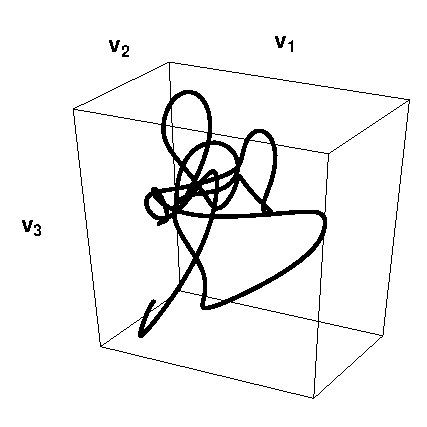
\includegraphics[width=0.40\textwidth, clip=true]
                    {../figs/ks22rpo033.50_04.045E2.eps}
~(\textit{b})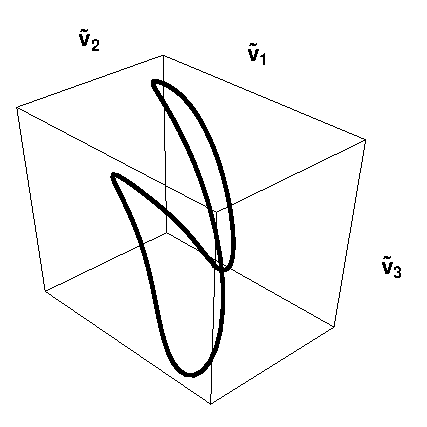
\includegraphics[width=0.40\textwidth, clip=true]
                     {../figs/ks22rpo033.50_04.045E2CM.eps}
\caption{
 A \rpo\ of the Kuramoto-Sivashinsky flow, traced for four periods
 $\period{p}$ and projected on
 (a) a stationary \statesp\ coordinate frame
 $\{v_1,v_2,v_3\}$;
 (b) a co-moving $\{\tilde{v}_1,\tilde{v}_2,\tilde{v}_3\}$
 coordinate frame, moving with the mean velocity
 $\velRel_p=\gSpace_p/\period{p}$.
(From \refref{SCD07}.)
}
\end{figure}
%%%%%%%%%%%%%%%%%%%%%%%%%%%%%%%%%%%%%%%%%%%%%%%%%%%%%%%%%%%%%%
%
A \emph{\rpo} is periodic in its mean velocity
$\velRel_p=\gSpace_p/\period{p}$ co-rotating frame,
\reffig{f:MeanVelocityFrame}, but in the stationary frame
its trajectory is quasiperiodic. A co-moving frame is helpful
in visualizing a single `relative' orbit, but useless for
viewing collections of orbits, as each one drifts with its
own group velocity. A simultaneous visualization of all
\rpo s as \po s we attain only by \emph{symmetry reduction},
to be undertaken in \refsects{s:Hilbert}{sec:mf}.

   % siminos/CLE/CLEsols.tex
% $Author$ $Date$

\subsection{\label{s:CLEsols} An example: Solutions of \cLe}

In the case of {\cLe}  the origin \EQV{0} is an \eqv\ of
\refeq{eq:CLe} for any value of the parameters. It is stable
for $0<\RerCLor<\rho_{1c}$ and unstable for
$\rho_{1c}<\RerCLor$, where\rf{FowlerCLE82}
\[
	\rho_{1c} = 1 + {(e+\ImrCLor)(e-\sigma \ImrCLor)}/{(\sigma+1)^2}
\,.
\]
At the bifurcation\rf{ruell73} a pair of eigenvalues crosses
the imaginary axis with imaginary part
\beq
	\omega_c = {\sigma (e + \ImrCLor)}/{(\sigma+1)}
\,,
\ee{eq:omegaCLE}
and a \emph{relative equilibrium} \REQV{}{1} with constant
angular velocity $\omega_c$ is born. For $\omega_c =0$ the
\reqv\ degenerates to an \SOn{2}-orbit of \eqva. As the
existence of a \reqv\ in a system with \SOn{2} symmetry is
the generic situation, we follow \refref{BakasovAbraham93}
and set $\ImrCLor=0$ and $e \neq 0$.

To find the location of the \reqv\ it is convenient to work
\JFGedit{in} polar coordinates
\beq
(x_1,x_2,y_1,y_2,z) =
    (r_1 \cos\theta_1,r_1\sin\theta_1,
     r_2\cos\theta_2,r_2\sin\theta_2,z)
\,,
\label{eq:CartToPol}
\eeq
where $r_1 \geq 0 \,,r_2 \geq 0$.
\JFGedit{The} \CLe\ \refeq{eq:CLe} take \JFGedit{the} form
\[ %\beq
\left(
\begin{array}{c}
\dot{r}_1\\
\dot{\theta}_1\\
\dot{r}_2\\
\dot{\theta}_2\\
\dot{z}
\end{array}
\right)
=
\left(
\begin{array}{c}
 -\sigma\left(r_1 - r_2\cos\theta\right) \\
 -\sigma\frac{r_2}{r_1}\sin \theta  \\
 -r_2 + r_1\left((\rho_1-z)\cos \theta - \rho_2 \sin\theta\right)\\
  e  + \frac{r_1}{r_2}\left((\rho_1-z)\sin\theta +\rho_2 \cos\theta\right)\\
 -b z + r_1 r_2\cos\theta
\end{array}
\right)
,
\] %\ee{eq:PolarCLe}
For
rotationally invariant flows the dynamics depends only
on the relative angle $\theta = \theta_1-\theta_2$
(\JFGedit{which} is why one speaks of `relative' equilibria).
This observation enables us to recast the \cLe\
in the  4-dimensional \reducedsp:
\beq
\left(
\begin{array}{c}
\dot{r}_1\\
\dot{r}_2\\
\dot{\theta}\\
\dot{z}
\end{array}
\right)
=
\left(
\begin{array}{c}
 -\sigma\left(r_1 - r_2\cos\theta\right) \\
 -r_2 + (\rho_1-z)r_1\cos \theta\\
  -e -\left(\sigma\frac{r_2}{r_1}
 +(\rho_1-z)\frac{r_1}{r_2}\right)\sin\theta\\
 -b z + r_1 r_2\cos\theta
\end{array}
\right)
\label{eq:PolarCLeTheta}
\eeq
where we have set $\rho_2=0$. The full 5-dimensional evolution can be
regained by integrating the two driven `reconstruction' equations:
\beq
\left(
\begin{array}{c}
\dot{\theta}_1\\
\dot{\theta}_2
\end{array}
\right)
=
\left(
\begin{array}{c}
-\sigma\frac{r_2}{r_1}\sin\theta  \\
 e + (\rho_1-z)\frac{r_1}{r_2}\sin\theta
\end{array}
\right)
\,.
\label{eq:PolarCLeAngles}
\eeq
In general $\theta_1$ and
$\theta_2$ change in time, but for the \reqva\ the
difference between them is constant.
The condition for a \reqv\ is that all
time derivatives in \refeq{eq:PolarCLeTheta} vanish, while
$\dot{\theta}_1=\dot{\theta}_2\neq 0$ (if
$\dot{\theta}_1=\dot{\theta}_2=0$ we have a group orbit
of \eqva\ instead).
The \reqv\
$\REQV{}{1}$ is given by
\bea
(r_1,r_2,\theta,z) &=&
\left(\sqrt{b \,(\rho_1-d)},  \sqrt{b d \,({\rho_1}-d}),
     \cos^{-1}({1}/{\sqrt{d}}),  \rho_1-d
\right)
\,,
\label{eq:E1-PC}
\eea
where $d=1 + {e^2}/{(\sigma +1)^2}$, and
its angular velocity is
\beq
\dot{\theta}_{i}
= {\sigma e}/{(\sigma + 1)}
\,,
\label{eq:REQV1veloc}
\eeq
with period
$\period{{\REQV{}1}}= 2\pi (\sigma + 1)/\sigma e$.
For the parameter values \refeq{eq:CLeR}, the \reqv\ is at
\beq
\ssp_{\REQV{}1} = (r_1,r_2,\theta,z) =
     (8.48527,
      8.48562,
      0.00909,
      26.9999)
\,,
\label{eq:Q1}
\eeq
rotating with the period $\period{{\REQV{}1}}=69.115$.\ES{Period feels too large, 
I'll double check in my notebooks.}

As $\RerCLor$ is increased,  a secondary bifurcation from
\REQV{}{1} results in a \emph{\rpo} \refeq{RPOrelper1}, or,
more precisely, in the quasiperiodic 2-frequency
\emph{modulated traveling wave}\rf{Krupa90}.
Calculation of \JFGedit{the} \REQV{}{1} stability eigenvalues
\PublicPrivate{}{
(see \ref{s:StabReq} for a calculation of stability of
\reqva\ in equivariant variables)
    } %end \PublicPrivate{}{
yields a weakly unstable spiral-out
\eqv\
\beq
(\eigExp_{1,2},\eigExp_3,\eigExp_4)
= (0.0938 \pm 10.1945 i,-11.0009,-13.8534)
\,.
\ee{eq:CLeREQBstab}
With further increase in $\RerCLor$ the dynamics turns
chaotic, with \JFGedit{an} infinity of unstable {\rpo s}. Large numbers of
these can be computed by methods described
elsewhere\rf{SCD07,SiminosThesis}.

The role of \JFGedit{the} above exact invariant solutions is illustrated by the
portrait of \cLf\ \statesp\ in  \reffig{fig:CLE}, with the
\reqv\ \REQV{}{1} and three repetitions of \JFGedit{the} \cycle{01} \rpo\
superimposed over a generic chaotic orbit. Repeats of
\cycle{01} \JFGedit{trace out a torus ergodically} , so in a system with
a $1$-dimensional continuous symmetry the organizational
blocks of a strange attractor are circles (\reqva) instead of
points (\eqva), and partially hyperbolic tori (\rpo s)
instead of closed loops (\po s). It is difficult to
understand the geometry of the flow by looking at such tori.

The large imaginary part of $\eigExp_{1}$ in
\refeq{eq:CLeREQBstab} implies that the simulation has to be
run up to time of order of at least 70 for the strange
attractor in \reffig{fig:CLE} to start filling in. Dynamics
is organized by the interplay of the stable and unstable
manifolds of \eqv\ \EQV{0} and \reqv\ \REQV{}{1}, but the
symmetry-induced drift along the direction of rotation blurs
the picture and the notion of recurrence becomes relative. In
what follows, it is this confusing situation (as well as the
theoretical fact\rf{Cvi07} that dynamical zeta functions have
their support on \rpo s) that motivates the search for
effective methods to project the dynamics onto a \reducedsp.


\section{\label{s:symRedGeneral} Symmetry reduction methods}
    \input symRedGeneral

\section{\label{s:Hilbert} Hilbert polynomial bases}
    \input Hilbert

\section{\label{sec:mf} Moving frames}
    \input movingFrames
    \input mfReqb
    \input mfLocal
    \input slice


\section{Conclusions}
    \input conclusions

\section*{Acknowledgements}
 Davidchack, Mitchell, Halcrow, Gibson, Barkley, ... Rowley(?)

% Specify following sections are appendices. Use \appendix* if there
% only one appendix.
\appendix

\section{\label{s:StabReq} Stability of \reqva}
    \input stabReqva

% \bibliographystyle{elsarticle-harv}
\bibliographystyle{elsarticle-num}
\bibliography{../bibtex/siminos}

% remove this when all problems have been fixed
    \newpage
    \input 05fixMe
    \input flotsam
\end{document}
